\documentclass[10pt,letterpaper]{article}
\usepackage[latin1]{inputenc}
\usepackage{amsmath}
\usepackage{amsfonts}
\usepackage{amssymb}
\usepackage{graphicx}
\usepackage{parskip}
\usepackage{todonotes}
\usepackage{url}


\newtheorem{example}{Example}[section]
\newtheorem{definition}{Definition}[section]
\newtheorem{remark}{Remark}[section]
\newtheorem{discussion}{Discussion}[section]
\newtheorem{excercise}{Excercise}[section]
\newtheorem{algorithm}{Algorithm}[section]

\DeclareMathOperator{\argmin}{arg\,min}
\DeclareMathOperator{\argmax}{arg\,max}
\DeclareMathOperator{\logsumexp}{logsumexp}

\newcommand{\set}[1]{\{#1\}}
\newcommand{\G}{\mathcal{G}}
\newcommand{\T}{T}

\title{Draft Technical Notes on BayesDB}

\begin{document}

\maketitle

\begin{abstract}
This document presents a probability-theoretic (but not necessarily
Bayesian) description of what it could possibly mean to ``have a model
of a data table'', and to ``learn a model of a data table''.  The goal
is to set the terms in which the interfaces to and semantics of
BayesDB operations may be described and discussed.
\end{abstract}

\section{Preface}

There are several things this document is not.

\paragraph{This is not a software spec.}  That is left to be
written in software.  If this document has served its purpose, the
software spec would reference it for conceptual background.  In
paricular, a software interface may depart from the interfaces of
Sections~\ref{sec:non-adaptive_gpm}~and~\ref{sec:adaptive_gpm} in
a few places.  For example:
\begin{itemize}
\item Specifying generation of multiple IID samples from the same
  distribution as a bulk operation for efficiency.
\item Specifying a particular data representation for collections of cells.
\item Possibility meriting more serious discussion: Intentionally
  restricting the class of questions that population models are
  expected to be able to answer, to prevent client analyses from
  relying on rare capabilities.
\end{itemize}

\paragraph{This is not a BQL syntax spec.}  There is squish room
in the interpretation of BQL queries against this interface.  For
example, should PREDICTIVE PROBABILITY condition on the data present
in the other cells of the row, on the row's identity, or both?  What
to make syntactically convenient is about anticipating user needs and
matching them to model capabilities; the authors expect this process to be
iterative.

\paragraph{This is not a Bayesian manifesto.}  Present nomenclature
notwithstanding, BayesDB has no reason to impose a Bayesian philosophy
of induction or learning on either its users or the implementors of
its population models.  Probability theory enters into BayesDB and
this document because it's the best formalism the authors know for
what it means to have a quantitatively incomplete model of something.
That happens in two places in BayesDB: any given population model is
expected to be incomplete; and the results of learning a population
model from observations may be incomplete (i.e., represent a
probability distribution over possible learned explanations).

\todo[inline]{Missing data.  Should explicitly say somewhere that
  missing data values are treated as ``no observation'', rather than
  observing a sentinel and forcing the GPM to deal with it.}

\section{Overview: Generative Population Models and the BayesDB Minimal Modeling Language}
\label{sec:overview}

BQL programs are executed against a set of ambient data
\textit{generative population models} (GPMs).  A GPM is assoicated
with a table in the database, which represents individuals observed
from that population.\footnote{Perhaps partially observed, if some cells in the
  table are null.} These generative population models are provided by
BayesDB based on modeling schemas and inference programs written in
the BayesDB Minimal Modeling Language.

\subsection{Generative Population Models}

Formally, a GPM is a probability distribution on unbounded-size
populations of individuals (which correspond to rows), with some fixed
set of attributes (which correspond to columns). A ``population'' is
an inherently unordered collection, so the distribution is taken to be
exchangeable.

\begin{example} \label{ex:normal_gpm} A Pretty Normal Generative Population
Model

Consider the following GPM on $D$-dimensional members of
a population $\mathbf{X}$: The individuals $\mathbf{X_i}$ are taken to
be independently identically distributed according to a mixture of two
normal distributions

\[ p_\mathbf{X_i}(x) = w_1\mathcal{N}(x;\mu_1,\Sigma_1) +
 w_2\mathcal{N}(x;\mu_2,\Sigma_2) \]

with fixed parameterization $(w_1, \mu_1, \Sigma_1, w_2, \mu_2, \Sigma_2)$.
\end{example}

While the GPM of Example~\ref{ex:normal_gpm} is valid, in that it is a
probability distribution on arbitrary-size populations, it is not
particularly interesting, because the individuals are independent and
the parameterization is fixed.\footnote{One plausible scenario in
  which such a ``fixed'' GPM can arise is by learning the model
  externally from BayesDB.  A user may decide to import such a GPM
  into BayesDB, without providing a hook for BayesDB to adapt it.}

In typical applications we are interested in \textit{learning the GPM
  from data}. For example, this might be learning the specific
parameters $\theta$ given a fixed generative process $M_i$, or
learning the generative process $M_i$ from some fixed model class
$\mathcal{M}$, or even learning the model class itself $\mathcal{M}$
from a set of competing model classes $\set{\mathcal{M}_k}$.  BayesDB
enables this with its notion of \emph{adaptive generative population
  models}, formalized in
Sections~\ref{sec:formalism-adaptive-gpm}~and~\ref{sec:formalism-incremental-gpm}
and specified in Section~\ref{sec:adaptive_gpm}.

\begin{example}
The GPM from Example~\ref{ex:normal_gpm} becomes adaptive if we take
the parameterization $(w_1, \mu_1, \Sigma_1, w_2, \mu_2, \Sigma_2)$ as
unknown and supply some scheme for inferring it from the observed
data.  Maximum likelihood estimation, posterior inference (exact or
approximate) in the presence of some prior, or any other deterministic
or stochastic procedure is permissible.  Different procedures lead to
different adaptive models, which in turn yield different answers to
queries.
\end{example}

We speak of \emph{generative} population models because we want a
joint probability distribution on all attributes of an individual, for
example to be able to impute arbitrary missing features, or synthesize
populations of hypothetical individuals from the model.  There are,
however, many techniques for modeling relationships between attributes
of an individual.  To be able to take advantage of these methods,
BayesDB admits the notion of a \emph{conditional GPM} that treats some
attributes as unmodeled inputs, and specifies a probability
distribution on other attributes (see Section~\ref{sec:generators} for
details).  The BayesDB Minimal Modeling Language
(Section~\ref{sec:mml}) permits specifying complete GPMs as directed,
acyclic compositions of such objects (on the columns).

\begin{example}
Regression (linear, logistic, or otherwise) and classification methods
are canonical instances of conditional GPMs, predicting the dependent
variable from the independent ones.
\end{example}

\subsection{The Minimal Modeling Language}
\label{sec:mml}

The BayesDB Minimal Modeling Language (MML) provides a framework for
associating various GPMs with data tables stored in BayesDB, and
adapting them to the data (learning), if applicable.

The MML includes a \textit{default adaptive generative population
  model} which defines a distribution over a collection of
\textit{GPMs from a default class} using a hierarchal, semi-parametric
Bayesian model derived from CrossCat.

\begin{example} \label{ex:crosscat} CrossCat

A cross-categorization of a data table $\mathbf{X}$ with $D$ columns and $N$ 
rows is
a partition of the columns $(X_1,\dots,X_D)$ into blocks called \textit{views}.
In each view, we have a partition of the rows $(X_1^{i},\dots,X_D^{i})_{i=1}^N$
into blocks called \textit{categories}.

\begin{figure}[ht]
    \centering
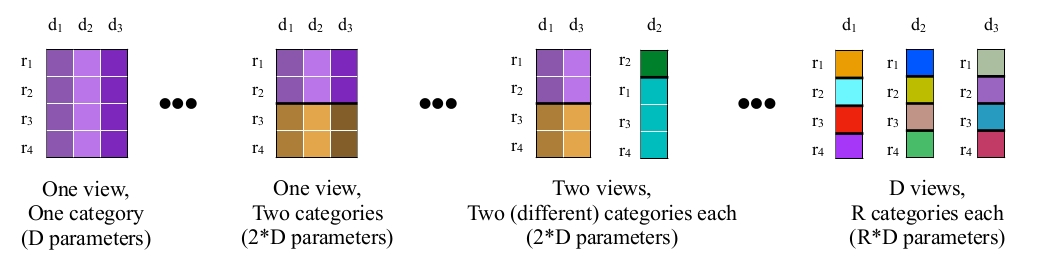
\includegraphics[width=0.8\textwidth]{cc.jpeg}
\caption{Some possible cross-categorizations of a table with 3 columns
  and 4 rows.  Any two cells with different colors are taken to be
  independent conditioned on the latent structure.}
\label{fig:cc}
\end{figure}
The collection of all possible column/row partitions $j$ of
$\mathbf{X}$, with their associated component parameters $\theta$,
defines a GPM class:

$\mathcal{M}_\textbf{X} = \set{CC_j^{\theta} \text{ : cross-cat of } \mathbf{X}
\text{ with partition } j \text{ and component model params } \theta}$.

A member of the CrossCat GPM class is a particular
cross- categorization with partition $j$ and component parameters
$CC_j^{\theta^*}$.  Adding a prior over these possible structures
defines an adaptive generative population model.
\end{example}

Unlike Example~\ref{ex:normal_gpm}, the latent information of the GPM
in Example~\ref{ex:crosscat} is structurally dependent on
the statistical population it has produced $\mathbf{X}$. Observing more
generated members $\mathbf{X} \to
\mathbf{X}'$ means the GPM class under consideration grows from
$\mathcal{M}_\textbf{X}$ to $\mathcal{M}_\textbf{X'}$, as both the number of
possible cross-categorizations $j$ and the dimensionality of the vector of
latents $\theta$ increase.

\todo[inline]{The reason I am being so pedantic about this construction is to
explicate various design choices when simulating, sampling, and running
posterior inference. In particular we are going to have to break down the latent
structure into ``global'' vs ``row-related'' latents to differentiate between
observed and hypothetical members.}

The default adaptive GPM is not obliged to model all columns jointly by
positing some GPM from the CrossCat class. The MML includes modeling
instructions for describing dependence constraints, and specifying a
compositional, directed-acyclic network of arbitrary GPMs implemented by a user.
It also includes inference instructions for initializing adaptive GPMs and
performing updates of the posterior distribution on GPMs.

The MML is thus a complete (but sub-Turing) probabilistic programming language
that interoperates with queries written in BQL. The set of primitive GPMs can be
extended by loading foreign GPMs written in VentureScript or Python, and can be used to
transparently integrate models from disparate probabilistic programming
languages such as Stan and statistical computing environments such as R. Because
BQL programs only depend on the statistical data types of the columns, the
underlying modeling technologies, GPM assumptions, and inference tactics can be
changed without invalidating end-user data analysis workflows.

\section{Interface for Generative Population Models} \label{sec:generators}
A \textit{generative population model} is a probabilistic model of a data
generating process and a statistical population that it has produced. It is
informative to think of this statistical population as an infinite table
$\mathbf{X}$ with a finite number of columns $D$ (representing attributes) and
an infinite number of rows (representing members of the population). A finite
number of rows $r_i \in
\set{1,\dots,N}$ are actually observed, so $\mathbf{X}$ is stored in BayesDB as
an $N \times D$ table. Hypothetical members may be referenced by any other row index,
for example by drawing a random real row index
$r^*\sim U[0,1]$.

Generative population models provide the primitive statistical inferences that
are used by BayesDB to implement inferential queries in BQL. To support all of
BQL, a GPM must provide the ability to \textbf{sample from} and \textbf{evaluate
the log density of}\footnote{With respect to counting measure for variables of
discrete statistical types and Lebesgue measure for continuous.}
all possible marginal distributions subject to equality
constraints for arbitrary subsets of variables.

\subsection{Non-Adaptive GPMs}
\label{sec:non-adaptive_gpm}

Since non-adaptive GPMs are by assumption IID on the individuals in
the population, they admit a simpler interface than adaptive ones.  As
such we present it first, and defer the generalization to
Section~\ref{sec:adaptive_gpm}.

\begin{enumerate}

\item \texttt{$\G$ = initialize(schema = $\Lambda$)}

    Initialize a GPM with the given schema, and return the resulting GPM
    $\G$.

    Each GPM is initialized with a \textit{schema} $\Lambda=$\path{(typed-
    outputs, typed-inputs, body)}. The \path{typed- outputs} component specifies
    the column indexes and statistical types of each column that the GPM will be
    responsible for generating. The \path {typed-inputs} component specifies the
    indexes and statistical types of columns that the GPM can read
    from.  If this set is non-empty, the GPM is \emph{conditional}.
    The \path{body} is a GPM-specific blob (opaque to BayesDB) that contains any
    desired configuration information.

\item \texttt{$\vec{s}$ =
    simulate($\G$, row = $i$, targets = $\set{c_j}_{j=1}^{|T|}$, givens
    = $\set{(c_k, x_{ik})}_{k=1}^{|G|}$)}

    Generate a sample from the specified conditional distribution on columns:
    $$
    \vec{s} \sim p( \set{ \mathbf{X}_{ij} } |
    \set{ \mathbf{X}_{ik} = x_{ik} }, \G).
    $$

    The returned $\vec{s}$ is a $|T|$ dimensional vector.

\item \texttt{$\log p$ =
    logpdf($\G$, row = $i$, targets = $\set{(c_j, x_{ij})}_{j=1}^{|T|}$,
    givens = $\set{(c_k, x_{ik})}_{k=1}^{|G|}$)}

    Evaluate the log probability density of the specified conditional
    distribution on columns at a target point:

    $$
    \log p = \log p( \set{ \mathbf{X}_{ij} = x_{ij} } |
    \set{ \mathbf{X}_{ik} = x_{ik} }, \G).
    $$

    The density is with respect to a product of counting and Lebesgue
    measures, correspoding to discrete and continuous statistical
    types for the relevant columns.  The distribution is interpreted
    as marginalizing out all random variables that are not mentioned.

\end{enumerate}

The column indexes $c_j, c_k$ referred to above must refer to columns
present in the table---the MML does not have a notion of hypothetical
columns.  Further, the \texttt{target} indexes must be a subset of the
columns in the \texttt{typed-outputs} of the GPM $\G$, and
the \texttt{given} indexes of each query must be a superset of the
\texttt{typed-inputs} of the GPM $\G$.  Note: A client may
specify some of the \texttt{typed-outputs} as \texttt{given} in any
given query.  Doing so picks out a conditional version of the output
distribution.

The row index $i$ may either refer to an individual in the
table, or a hypothetical individual.  In the former case, the
distribution being sampled or assessed is taken as conditional on
whatever latent information is available about that individual, but
\emph{not on any attributes stored in the table} except as repeated in
the \texttt{givens}.  In the latter case, the distribution is taken to
refer to a fresh individual (i.e., marginalizing out any
per-individual latent structure).

\subsection{Formalism for Adaptive GPMs}
\label{sec:formalism-adaptive-gpm}

As outlined in Section \ref{sec:overview}, some GPMs can be learned
from observations $\set{\mathbf{X}_{ij} = x_{ij}}$ of a statistical population
$\mathbf{X}$.  Since we permit the learning to itself be stochastic,
the general case is a family of conditional probability distributions
(of learning results) for all possible sets of observations.  Formally:

\begin{definition} Adaptive Generative Population Model

An \emph{Adaptive Generative Population Model} over a class of GPMs
$\{\G_\alpha\}$ is a family of conditional probability distributions
$\Pi(\G_\alpha|\{\mathbf{X}_{ij} = x_{ij}\})$, for all possible
observation sets $\{x_{ij}\}$.
\end{definition}

\begin{example} Linear Regression

Linear regression (with a fixed noise model $\mathcal{E}$) can be viewed as a
conditional adaptive GPM over the class of non-adaptive GPMs
parameterized by the possible regression coefficients $\vec\beta_j$.
For a given set of input columns, defining inputs $\vec x$, and output column $y$,
the update rule corresponding to maximum likelihood estimation would be

\[ \vec\beta^*|\{\vec x_i, y_i\} = \argmax_{\vec\beta^*} \sum_i
   p_{\mathcal{E}}(y_i | \vec x_i^T \vec\beta^*). \]

The {\tt simulate} and {\tt logpdf} methods would refer to the
noise distribution around the predicted value for $y$.
\end{example}

\begin{example} Exact Bayesian Adaptive GPMs

For any GPM class $\{\G_\alpha\}$, an \emph{exact Bayesian adaptive
  generative population model} is given by a prior
$\Pi(\G_\alpha)$ over
$\{\G_\alpha\}$, and the adaptation rule

\[ \Pi(\G_\alpha|\set{\mathbf{X}_{ij} = x_{ij}}) \propto \Pi(\G_\alpha)
 p(\set{\mathbf{X}_{ij} = x_{ij}}|\G_\alpha), \]

where $p(\cdot|\G_\alpha)$ is the probability of the observed data under
the particular GPM $\G_\alpha$. \label{ex:exact-bayes}
\end{example}

\subsection{Incremental Adaptive GPMs}
\label{sec:formalism-incremental-gpm}

The desired adaptation rule of an adaptive GPM (such as the exact
Bayesian rule of Example~\ref{ex:exact-bayes}) may not always be
tractable to compute.  BayesDB permits adaptive GPMs to expose a
time-accuracy tradeoff in the form of incremental adaptation, where
the client is invited to select the amount of computational resources
they are willing to commit, and rewarded for greater commitment with a
superior quality of adaptation.  Formally this involves adding a ``fuel''
parameter to the adaptation rule:

\begin{definition} Incremental Adaptive Generative Population Model
\label{def:incremental-adaptive}

An \emph{Incremental Adaptive Generative Population Model} over a
class of GPMs $\{\G_\alpha\}$ is a family of conditional probability
distributions $\Pi_n(\G_\alpha|\set{\mathbf{X}_{ij} = x_{ij}})$, for all
possible observation sets $\{x_{ij}\}$ and all positive integers $n$,
where increasing $n$ represents increasing computational
cost.\footnote{In Section~\ref{sec:adaptive_gpm} we will specify a
  somewhat more flexible interface to learning than iterating a single
  transition operator, but spelling that out at this point would be
  needlessly notationally cumbersome.}
\end{definition}

\begin{example} Bayesian Markov Adaptive GPMs

For any GPM class $\{\G_\alpha\}$, a \emph{Bayesian Markov adaptive
  generative population model} is given by a prior
$\Pi(\G_\alpha)$ over
$\{\G_\alpha\}$, a data-dependent transition operator
$\T_{\{x_{ij}\}}$ over $\{\G_\alpha\}$, and
an adaptation rule that consists of iterating $\T$:

\[ \Pi_n(\G_\alpha|\set{\mathbf{X}_{ij} = x_{ij}}) = \T_{\set{x_{ij}}}^n 
\Pi(\G_\alpha). \]
\label{ex:markov-bayes}
\end{example}

This will be \emph{asymptotically Bayesian} if the transition operator
converges to the true posterior, that is if

\[ \lim_{n\to\infty}D_{KL}\Big(\Pi^*(\G_\alpha|\set{\mathbf{X}_{ij} = x_{ij}}) \Big\| \Pi_n(\G_\alpha|\set{\mathbf{X}_{ij} = x_{ij}})\Big) = 0, \]

where $\Pi^*(\G_\alpha|\set{\mathbf{X}_{ij}=x_{ij}}) \propto 
\Pi(\G_\alpha) p(\set{\mathbf{X}_{ij}=x_{ij}}|\G_\alpha)$
as in the exact Bayes case (Example~\ref{ex:exact-bayes}).
If the true data distribution falls into the hypothesis class given by
the prior $\Pi$, this will also be \emph{asymptotically consistent} in
the usual sense.

Since non-incremental adaptive GPMs are a special case of incremental
ones, we will make the assumption of incrementality in the rest of
this document, and omit the adjective.

\subsection{Interface for Adaptive GPMs}
\label{sec:adaptive_gpm}

The interface for (potentially incremental) adaptive GPMs is outlined
below.  The key differences from the interface to non-adaptive GPMs
defined in Section~\ref{sec:non-adaptive_gpm} are as follows:

\begin{itemize}
\item We add \texttt{incorporate} and \texttt{remove} methods to
  manipulate the set of observed individuals on which the adaptive GPM
  is taken to be conditioned.
\item We add an \texttt{infer} method to control expenditure of
  computation on incremental adaptation.
\item We generalize the \texttt{simulate} and \texttt{logpdf} methods
  to permit querying and conditioning on multiple rows, since the
  joint distribution on several rows need no longer be the product of
  the corresponding marginal distributions.
\end{itemize}

Note: An adaptive GPM can be used as a non-adaptive GPM by
marginalizing out the distribution over the class it is supposed to
adapt over.

\begin{enumerate}

\item \texttt{$\G$ = initialize(schema = $\Lambda$)}

    Initializes an adaptive GPM with the given schema \texttt{$\Lambda$ =
    (typed-outputs, typed-inputs, body)}.  This is identical with the
    \texttt{initialize} operation for non-adaptive GPMs.  The distribution $\Pi$
    on adaptations is taken to be conditioned on the empty set of observations
    $\Pi(\G_\alpha|\{\})$.  In the Bayesian case, this would be the prior.

\item \texttt{$\vec{s}$ =
    simulate($\G$, targets = $\set{(r_j,c_j)}_{j=1}^{|T|}$, givens
    = $\set{(r_k, c_k, x_{r_kc_k})}_{k=1}^{|G|}$)}

    Generate a joint sample from the specified conditional
    distribution on cells.
    $$
    \vec{s} \sim p( \set{ \mathbf{X}_{r_jc_j} } |
    \set{ \mathbf{X}_{r_kc_k} = x_{r_kc_k} }, \G)
    $$

    Note that $\vec{s}$ is a $|T|$ dimensional vector of the simulated
    values for those cells.  As in the non-adaptive case
    (Section~\ref{sec:non-adaptive_gpm}), row indexes control conditioning
    or lack thereof on per-individual latent structure, but all conditioning
    on manifest structure is determined by the \texttt{givens}.
    
\item \texttt{$\log p$ =
    logpdf($\G$, targets = $\set{(r_j, c_j, x_{r_jc_j})}_{j=1}^{|T|}$,
    givens = $\set{(r_k, c_k, x_{r_kc_k})}_{k=1}^{|G|}$)}

    Evaluate the log probability density of the specified conditional
    distribution on cells at a target point.

    $$
    \log p = \log p( \set{ \mathbf{X}_{r_jc_j} = x_{r_jc_j} } |
    \set{ \mathbf{X}_{r_kc_k} = x_{r_kc_k} }, \G)
    $$

    As in the non-adaptive case, the density is with respect to a
    product of counting and Lebesgue measures, correspoding to
    discrete and continuous statistical types for the relevant
    columns.  The distribution is interpreted as marginalizing out all
    random variables that are not mentioned.

\item \texttt{$\G'$ = incorporate($\G$, value = $(i, j, x_{ij})$)}

    Record an observation $x_{ij}$ in the cell $\mathbf{X_{ij}}$.
    If there is no row $i$, create a new one.

    It is an error for the client to overwrite existing cells, or to insert values
    $x_{ij}$ incompatible with the schema $\Lambda$ (for example,
    providing data of the wrong type).

    Consecutive calls to \texttt{incorporate} (and \texttt{remove})
    should commute.  In the case of incremental GPMs, intervening
    \texttt{infer} is permitted to break commutativity.

\item \texttt{$\G'$ = remove($\G$, $(i, j)$)}

    Remove the observation $x_{ij}$ from the in cell $\mathbf{X_{ij}}$.
    Consecutive \texttt{remove} should exactly invert
    \texttt{incorporate} on the same cell.  In the case of incremental
    GPMs, intervening \texttt{infer} is permitted to change the
    result.  (That is, \texttt{incorporate}, \texttt{infer}, \texttt{remove}
    may be different from just the \texttt{infer}.)

\item \texttt{$\G'$ = infer($\G$, program = $\mathcal{P}$)}

    Adjust any internal latent state in accordance with the inference
    procedure specified in the program $\mathcal{P}$.  To BayesDB, the
    inference program is an opaque blob; the menu of accepted
    inference programs is expected to be designed in tandem with the
    \texttt{body} specified in the schema $\Lambda$.

    In the case where $\G$'s state is samples from the current state
    of a Markov chain, $\mathcal{P}$ would specify application of a
    transition operator.  If that operator were asymptotically
    Bayesian, each run of \texttt{infer} would improve the quality
    with which the distribution on sub-models $\{\G_\alpha\}$
    approximates the posterior.
\end{enumerate}

Note that the interface specified above is somewhat more flexible than
Definition~\ref{def:incremental-adaptive} given for incremental
adaptive GPMs.  In particular:

\begin{itemize}
\item Addition (and removal) of data may be interleaved with learning
  and querying.
\item A GPM may specify a menu of possible inference programs as
  options for learning, in which case the learned distribution on
  $\{\G_\alpha\}$ would depend on the sequence of arguments passed to invocations
  of \texttt{infer} (and how they are interspersed with
  \texttt{incorporate} and \texttt{remove}), rather than simply on
  their count as Definition~\ref{def:incremental-adaptive} suggests.
\end{itemize}

\subsection{Ensembling Adaptive GPMs}
\label{sec:ensemble}

If BayesDB inferences were based on a single instance of an adaptive
GPM, the inferences could arbitrarily suppress modeling
uncertainty. The MML provides users a generic \emph{GPM ensemble}
mechanism, that can be used for measuring and improving accuracy of
inferences.  In the language of Markov chains, the ensemble represents
a set of independent, parallel chains, which answers queries by simple
Monte Carlo over its constituents.

An ensemble of (adaptive, incremental) GPMs is itself an (adaptive,
resp.\ incremental) GPM.  The default ensemble implements the GPM interface of
Section~\ref{sec:adaptive_gpm}
as follows:

\begin{enumerate}
\item \texttt{$\mathcal{Q}$ = initialize(schema = $\Lambda$, count = S)}

    Accepts an additional \texttt{count} argument, to specify the size
    of the ensemble.  Operationally, initializes a collection of $S$
    GPMs with the schema $\Lambda$ (independently, if the
    initialization is stochastic).
    $$
    \mathcal{Q} = (\set{\G_s}_{s=1}^S, \mathbf{X_\mathcal{Q}})
    $$

    The schema and data store are shared across all GPMs in the
    ensemble.

\item \texttt{simulate} delegates to a uniformly random ensemble
  element $\G_k$.

    $$
    \vec{s} = \texttt{simulate} (\G_*,\dots) \text{ where }
    \G_* \sim U[\set{\G_s}]
    $$

  \todo[inline]{Maybe conditional simulation should weight the ensemble
    elements by how likely those conditions are in them?  It can, by
    invoking their logpdf methods.  This would worsen the asymptotic
    complexity of simulate, though.}

\item \texttt{logpdf} forms a Monte Carlo estimate of the expected density using
all of the GPMs in the ensemble.

    $$
    \log p = \logsumexp_s\texttt{logpdf}(\G_s) - \log S
    $$

\item \texttt{incorporate}, \texttt{remove}, and \texttt{infer} apply
  pointwise to all the GPMs in the ensemble.

\end{enumerate}

More elaborate methods such as likelihood weighting or particle
filtering ensembles are possible extensions.

\section{Derived Functions}

The operations \texttt{simulate} and \texttt{logpdf} are directly
accessible to BQL programs via the \texttt{SIMULATE} and
\texttt{PROBABILITY OF} syntax.  Other query functions may be
implemented generically in terms of \texttt{simulate} and
\texttt{logpdf}; though many of them may also have more efficient
short-cut implementations that are specific to the structure of a
given GPM.  This section defines the derived functions and sketches
their default implementations provided by BayesDB; a software
interface to GPMs should permit the GPM to override any of these
implementations with custom ones tailored to the model, as they may be
subtantially more efficient.

\todo[inline]{What time/accuracy knobs should be exposed in the
  interfaces?  I suppose that can be left to the software spec also.}

\subsection{Conditional Mutual Information}

\begin{definition} Conditional Mutual Information \todo{standard reference}

The \emph{conditional mutual information} (CMI) of two random variables $A$
and $B$ with respect to a third variable $C$ is the expectation, with
respect to $C$, of the mutual information of the conditional variables
$A|C$ and $B|C$.  In the discrete case this can be written as

    \begin{eqnarray*}
    I(A;B|C) & := &
        \sum_c p_C(c) \sum_{a,b} p_{A,B|C}(a,b|c) \log
            \frac{p_{A,B|C}(a,b|c)}{p_{A|C}(a|c) p_{B|C}(b|c)} \\
    &=& \sum_{a,b,c} p_{A,B,C}(a,b,c) \log
            \frac{p_C(c) p_{A,B,C}(a,b,c)}{p_{A,C}(a,c) p_{B,C}(b,c)}.
    \end{eqnarray*}

\end{definition}

In the context of the (notionally) infinite random table $\mathbf{X}$
induced by any given GPM $\G$,
BayesDB can estimate the joint conditional mutual information for any
three collections of cells $A$, $B$, $C$, itself in a population distribution
conditioned on given values $d$ for any fourth collection of cells $D$:

    \begin{align*}
    \set{(\hat{a}_j,\hat{b}_j,\hat{c}_j)}_{j=1}^n & \sim n \textrm{ iid samples from } p_{A,B,C|D=d} \\
    I(A;B|C,D=d) & \approx
        \sum_{\hat{a}_j,\hat{b}_j,\hat{c}_j} \log
         \frac{p_{C|D=d}(\hat{c}_j)
         p_{A,B,C|D=d}(\hat{a}_j,\hat{b}_j,\hat{c}_j)}
         {p_{A,C|D=d}(\hat{a}_j,\hat{c}_j) p_{B,C|D=d}(\hat{b}_j,\hat{c}_j)}
    \end{align*}

    The samples and log densities are computed by invoking
    \begin{align*}
    {\tt simulate}&(\G, {\tt targets} = A \cup B \cup C, {\tt givens} = (D, d)) \\
    {\tt logpdf}&(\G, {\tt targets} = C, {\tt givens} = (D, d)) \\
    {\tt logpdf}&(\G, {\tt targets} = A \cup C, {\tt givens} = (D, d)) \\
    {\tt logpdf}&(\G, {\tt targets} = B \cup C, {\tt givens} = (D, d)) \\
    {\tt logpdf}&(\G, {\tt targets} = A \cup B \cup C, {\tt givens} = (D, d))
    \end{align*}
    in the appropriate pattern.

\todo[inline]{Specify effort throttles and characterization of
  uncertainty (e.g., returning the entire set of $n$ point estimates)}
\todo[inline]{With an ensemble, there is a choice of whether to
  internally average the individual members' assessments, or to expose
  all of them for further uncertainty characterization (in any of
  several possible configurations)}

\begin{example} Mutual Information

The per-column mutual information available in BQL with the
\texttt{MUTUAL INFORMATION} syntax is a special case of CMI with
$C = D = \emptyset$ and $A = \set{*, c_1}$, $B = \set{*, c_2}$
singleton collections of cells of (the same) fresh individual's
attributes corresponding to the desired columns.
\end{example}

\subsection{Marginal Dependence Probability}

\begin{definition} Dependence Probability
\label{def:dep-prob}

The \emph{dependence probability} of random variables $A$ and $B$
under a probability distribution $\Pi$ over GPMs $\set{\G_\alpha}$
is the probability with respect to $\Pi$ that $A$ and $B$ are
dependent in $\G_\alpha$.
\end{definition}

We speak of \emph{marginal} dependence probability because we
marginalize out random variables other than $A$ and $B$.

BayesDB can estimate the dependence probability of two cells under an
ensemble GPM by querying each ensemble member for the (unconditional)
mutual information of those two cells and returning the proportion of
members where the result is non-zero (indicating dependence).

Note: Dependence probability is well-defined for a deterministically
adaptive GPM, but is always either zero or one (independent or
dependent).

\todo[inline]{The dependence probability of columns is the dependence
  probability of those cells for (the same) fresh individual.}

\todo[inline]{Can generalize to dep-prob between any two sets of
  cells, jointly; and/or dep-prob conditioned on any desired data}

\todo[inline]{Is there a meaningful concept of ``conditional
  probability of dependence'' which would correspond to ``conditional
  mutual information''?  For example, the probability over $c$ under
  the distribution $C$ that $A|C$ and $B|C$ are dependent at $C=c$?}

\todo[inline]{Dependence probability is not to be confused with
  confidence (in a frequentist sense) that things are independent in
  the posterior predictive.}

\subsection{Marginal Dependence Magnitude}

\todo[inline,color=red]{Dependence magnitude is slippery:}

We have consistently meant ``some normalized version of mutual
information'', but:
\begin{itemize}
\item Mutual information measures how informative one variable is
  about another; what people actually want when they ask for a
  magnitude of dependence is ``effect size''---how much can pushing
  one variable be expected to move another.  This is what correlation
  coefficients and regression coefficients try to get at.
\item Normalizing mutual information turns out to be non-trivial,
  because the definition is fuzzy in the continuous case---it always
  takes an infinite number of bits to exactly encode a continuous
  value, so information gain is a strange concept.
\end{itemize}

If we do mean ``some normalized version of mutual information'', the
default implementation is straightforward once we select a
normalization mechanism.  One historical choice would be the Linfoot
measure:\footnote{http://www.sciencedirect.com/science/article/pii/S001999585790116X}

\begin{align*}
r^2 = \sqrt{1 - \exp{(-2I_0)}}
\end{align*}

Linfoot is normalized between 0 and 1, but there are some questionable
properties.  For example, if $Y=g(X)$, Linfoot is not guaranteed to be
1 (easy to construct an example in the discrete case).  Moreover, feedback
from PPAML is that the z-matrices it produces are sparse and
uninsightful, and give the implication that continuous variables are
more dependent than categorical ones.

\todo[inline]{Thought: If we already have probability of dependence,
  magnitude of dependence may naturally read as ``assuming there is a
  dependence'', which would suggest excluding ensemble members for
  which the distributions register as independent from any averages
  involving magnitudes.  Do we want to do that?}

\subsection{Generative Similarity}

There are actually three different things that similarity of two
type-aligned collections of cells (e.g., two rows) might reasonably
mean:

\begin{itemize}
\item Probability of being marginally equidistributed (note: this is
  orthogonal to dependence)
\item Information-theoretic distance between marginal distributions
\item Domain-semantic distance between marginal distributions
\end{itemize}

The first of these can be defined and computed similarly to dependence
probability (definition~\ref{def:dep-prob}), except with K-L
divergence instead of mutual information.

The second of these can just be the K-L divergence, perhaps
symmetrized, normalized, and/or smoothed (e.g., Jensen-Shannon
divergence\footnote{https://en.wikipedia.org/wiki/Jensen-Shannon\_divergence},
or its square root, which has the additional advantage of being a metric).

The third of these is pretty obnoxious, because it calls for distances
between distinct data items.  It may be possible to make a reasonable
interface for metrics on numerical variables, but similarity of
different categorical values is likely to be a problem.  On the other
hand, the information-theoretic measures all treat any two distinct
end values as maximally dissimilar.

In any case, similarity is definable for any two collections,
admitting arbitrary fixed-value conditions, and admitting a
``conditioned'' variant that asks whether the desired variables are
always similar for all possible values that might be conditioned upon
(or giving the expectation of their similarity over the possible
conditioning values).

\subsection{Imputation}

The intent of imputation for some cell(s) $A$ is to return a single
(vector) value that summarizes the information in the (joint)
distribution on $A$, and the confidence that this summary is ``good''.

If all of $A$ is discrete, this has a natural interpretation as
``return the max a-posteriori value, with confidence its
probability.''  If continuous variables are involved, however, things
get a bit fuzzier.

\subsubsection{Credible Sets}

Imputation can be viewed as a version of the Bayesian credible set
problem.  Valid answers to the credible set problem are pairs of a set
of values and a lower bound on the probability mass contained in that
set.  Desired answers are small sets and high mass bounds.  The
discrete solution suggested above obeys the constraint that the
returned set must be a singleton, and optimizes the mass bound subject
to that.

One can therefore imagine queries that constrain either the size of
the set and request the location and the best confidence (impute with
confidence), or constrain the confidence and request the location and
the best size (impute with error estimate), or constrain both and
request the location or failure.  (Constraining the location is
assessment, not imputation).  In the multidimenional case, there is
also the issue of the shape of the set.  Natural choices for
continuous variables include balls under $L_1$ (Manhattan distance,
i.e. total error), $L_2$ (Euclidean distance), or $L_\infty$ (maximum
error), or various combinations thereof that treat different
dimensions non-uniformly; natural choices in the fully discrete case
include singletons, boxes, or no shape restriction (a list of
plausible tuples).

All of these queries are approximately answerable in terms of
\texttt{simulate}: draw a bunch of samples, find a set of the proper
shape, and report the fraction of them that it covered as the
confidence.  There may be some variations where one uses assessments
of the sample points rather than their count for some information,
especially in the discrete setting.  In low dimensions, quadrature
over assessment may also be competitive.

\subsubsection{Approximating Distributions}

Credible sets can be viewed as summarizing the distribution as uniform
over some shape and size of set, except for two not unrelated
considerations.  One is that interpreting a set as a uniform
probability distribution requires having a base measure (e.g.,
Lebesgue) and having that set's size in that measure be finite and
positive.  The other is in the performance metric: ``the mass
contained in the set'' can always be increased by enlarging the set,
whereas enlarging the support of a uniform distribution reduces its
density at the supported points and thus may reduce the accuracy with
which it approximates the target.

One can therefore consider a formulation of imputation as
approximating the true distribution with some unimodal one.  This
leaves open the choice of unimodal distribution class and the choice
of distance measure.  For any such choice, the result is a
well-defined optimization problem.\footnote{This optimization
  formulation goes by the name ``variational inference'' when applied
  to approximating the posterior on latents with respect to K-L
  divergence.  Here we are approximating the posterior predictive
  distribution, with a to-be-chosen quality metric.}

BayesDB can approach all variants of imputation as approximation by
the following generic recipe: Draw some samples from the distribution
being approximated; fit a distribution from the approximating family
to them; estimate the desired distance metric (e.g., K-L divergence);
and report all the above.

Interface questions also arise:
\begin{itemize}
\item An imputation in this style produces two different error
  estimates: the dispersion of the approximating distribution, and its
  divergence from the true distribution.  How to surface both of them?
\item Allowing the user to bounding the confidence (in the sense of
  distance to the true distribution) still makes some sense, even
  though we would not be able to compensate for an exacting bound by
  supplying a broad prediction.
\item Does it make sense to allow the user to bound the dispersion of
  the approximating distribution (i.e., ``error tolerance'')?  Such a
  restriction would behave weirdly, in that it wouldn't always be
  binding.
\item If the divergence metric is taken to be K-L divergence, how to
  communicate it to the user?  I personally find actual divergence
  numbers pretty unintuitive, and they would not be normalized.  Is
  total variation distance any better?  Is there a Monte Carlo
  estimation procedure for it that we can rely on?
\end{itemize}

\subsubsection{Other Considerations}

\paragraph{Conditional Imputation}
Since we assume that a GPM can simulate and assess conditionally, we
can expose conditional imputation: ``Tell me about the value of $A$
assuming $B=b$.''  In fact, for a data cleaning application, one would
expect imputation of empty cells to be conditioned on the non-empty
cells in the same row.

\paragraph{Joint or Marginal Imputation}
If the values of multiple cells are called for, there is a choice
about whether to impute them marginally (i.e., each separately) or
jointly (i.e., one imputation summarizing the joint distribution on
those cells).  I don't know whether those are different for CrossCat,
but it's not hard to compute with examples of general distributions
where those two questions have different answers.

\subsection{Typicality}

There is no consensus in the field on what this ought to be, or on
what this ought to be useful for.  Decision: remove row and column
typicality for the public release, and possibly reconsider it in light
of reception and time.

\section{Open Issues}

\subsection{Identity Remapping}

The spec now identifies rows in the database with individuals in
the statistical population.  In principle, this need not be so---we can admit, e.g.,
a special (categorical) column that serves as an individual ID.  These can collide,
implying multiple observations of the same individual (so now the latents break
down into per-individual latents and per-observation latents); these can also be unknown,
implying identity inference.

Actually, come to think of it, I think that arrangement requires no
special provision by us: the user's GPM may treat a column in the
table as the identity of an individual.

\todo[inline]{Agreed?}

\subsection{Technical Aside On IID Rows}

\todo[inline]{Find a place for the ideas contained in this chunk of prize-winning text:}

The classical statistical framework generally assumes that all members of a
population are independent and identically
distributed.  \todo{Conditioned on parameters that are taken
to be unknown and adversarially set.} While a particular
generator is free to make any assumptions about its population, the IID
assumption is a strong one. The default generator (and almost any generator
being learned under the Bayesian framework) will usually assume that the rows
are not IID but exchangeably coupled. De Finetti's theorem guarantees that there
exists a mixture of random measures $\set{\G_\alpha}$ (which in most
cases is indexed by the latent state of the GPM) where the population is
conditionally IID.

$$p(\mathbf{X}) = \int_\alpha{(\Pi_{i=1}^Np(\mathbf{X}_i|\G_\alpha))d
\mathcal{Q}(\G_\alpha)}$$

The De Finetti measure $\mathcal{Q}$ is the object which defines a distribution
over the (fixed) measures (GPMs) that produce a statistical population. In this
sense, $\mathcal{Q}$ represents the adaptive GPM.

\subsection{Incorporating simulated data}

Incorporating data simulated from the current latent distribution is
cheap, at least in a Bayesian GPM, because it does not alter the
latent distribution.  However, if a client calls \texttt{simulate} and
then \texttt{incorporate}, the GPM has no proof that the item being
incorporated is the item that was simulated, so is called upon to do
more inference to reach the new posterior.  It seems advantageous to
be able to avoid this work, especially for the purpose of constructing
multi-row simulate from single-row simulate.

\begin{itemize}
\item Option: Specify simulate as auto-incorporating.  That is,
all simulations are implicitly part of a multi-row simulate unless
expressly undone.
\begin{itemize}
\item Pro: Natural definition of multi-row simulate in terms of single-row
\item But: Does not extend to logpdf
\item Pro: Avoids dirtying inference state as a simulate/incorporate cycle
  would
\item Undoing can be implemented by rollback at the DB level
\item Can still offer multi-row simulate and auto-forgetting simulate as
  alternatives/fast paths
\item Con: Multi-sample IID simulate becomes hairier
\item Con: Can't promise that simulate and logpdf do not modify the GPM
  (and that incorporate/remove/infer commute through simulates, which
  would not be true)
\end{itemize}
\item Option: Specify ``incorporate-just-generated'' as another
  interface method.
\item Option: Specify ``simulate-incorporating'' as an
  inference-avoiding fast path.
\end{itemize}

\appendix
\section{Stuff to revisit after the first public release}

\paragraph{Row/column typicality}
We might try to see whether early users want this, and whether it can
be defined sensibly.

\paragraph{Column similarity}
Idea: column similarity might usefully be the probability that those
cells of a fresh individual are identically distributed.  We can think
about whether to add this.

\end{document}
